\section{Design}

\subsection{Description/About}

Assignment for this project can be divided into these subtasks:
\begin{enumerate}
\item User input handling
\item Processing of DNS data
\item Exporting to a Syslog server
\end{enumerate}

\vspace{1cm}
\textbf{User input handling}

This task includes argument parsing, asserting for certain input conditions and general execution configurations.

\vspace{1cm}
\textbf{Processing of DNS data}

While the processing of DNS messages could be considered as the primary task of this project, several prior processing steps are required for an effective DNS analysis.
Before it becomes possible to parse DNS messages on the application layer, application needs to descend layer by layer and test for various conditions.
First, L2 or the link layer protocols are parsed, with support of Ethernet and Linux Cooked Header frames. Second, L3 or network layer protocols are parsed (IPv4 and IPv6).
Then, L4 or transport layer protocols are parsed (TCP and UDP). Finally, L7 or the application layer is unveiled and DNS data can be parsed.

\vspace{0.5cm}

All of the DNS communication is carried in a single format called \textit{a message}.
To properly parse \textit{a message}, it's structure needs to be understood.

\begin{figure}[h]
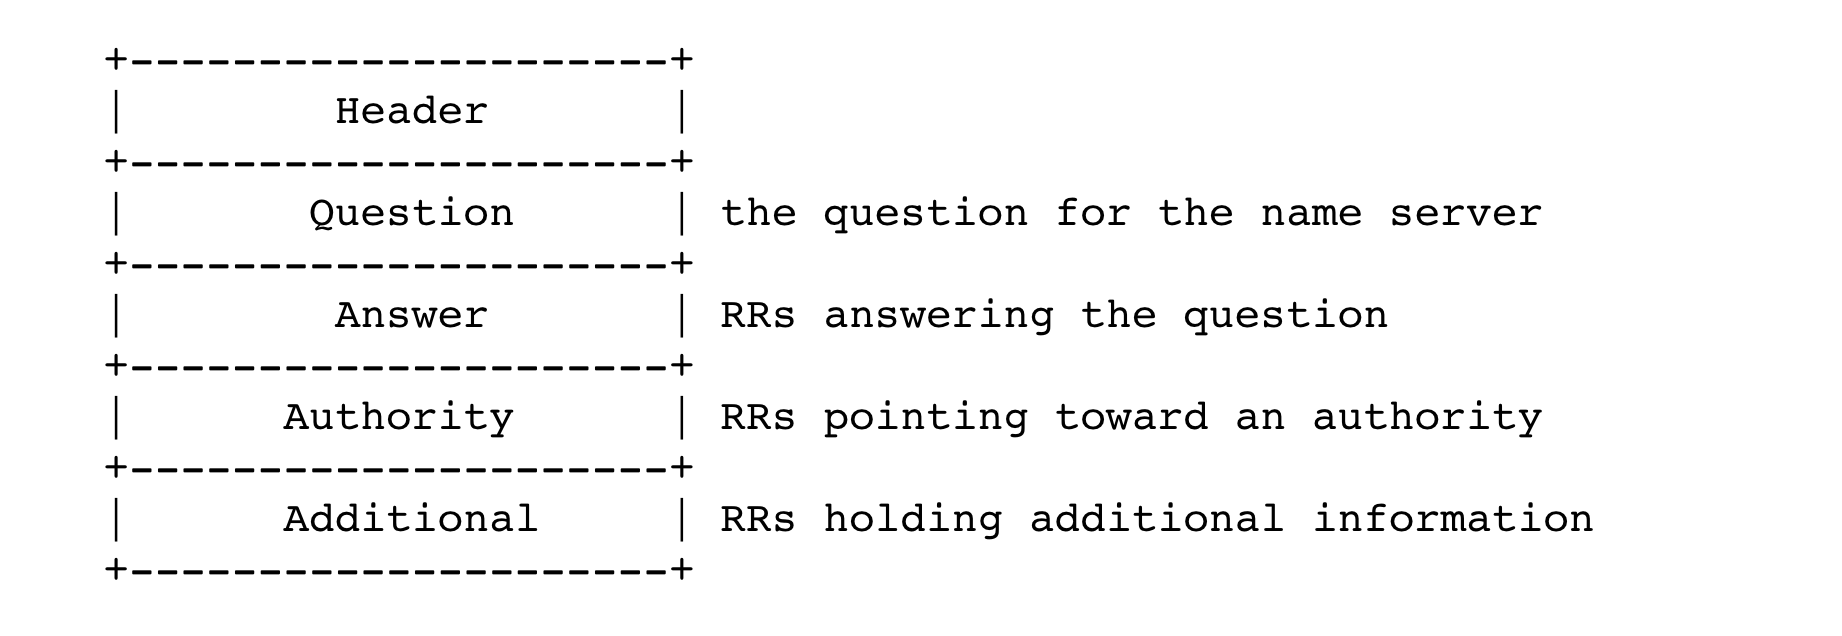
\includegraphics[width=16cm]{dns-message-structure}
\centering
\caption{4.1. Format | RFC 1035}
\end{figure}

\pagebreak

\begin{figure}[h]
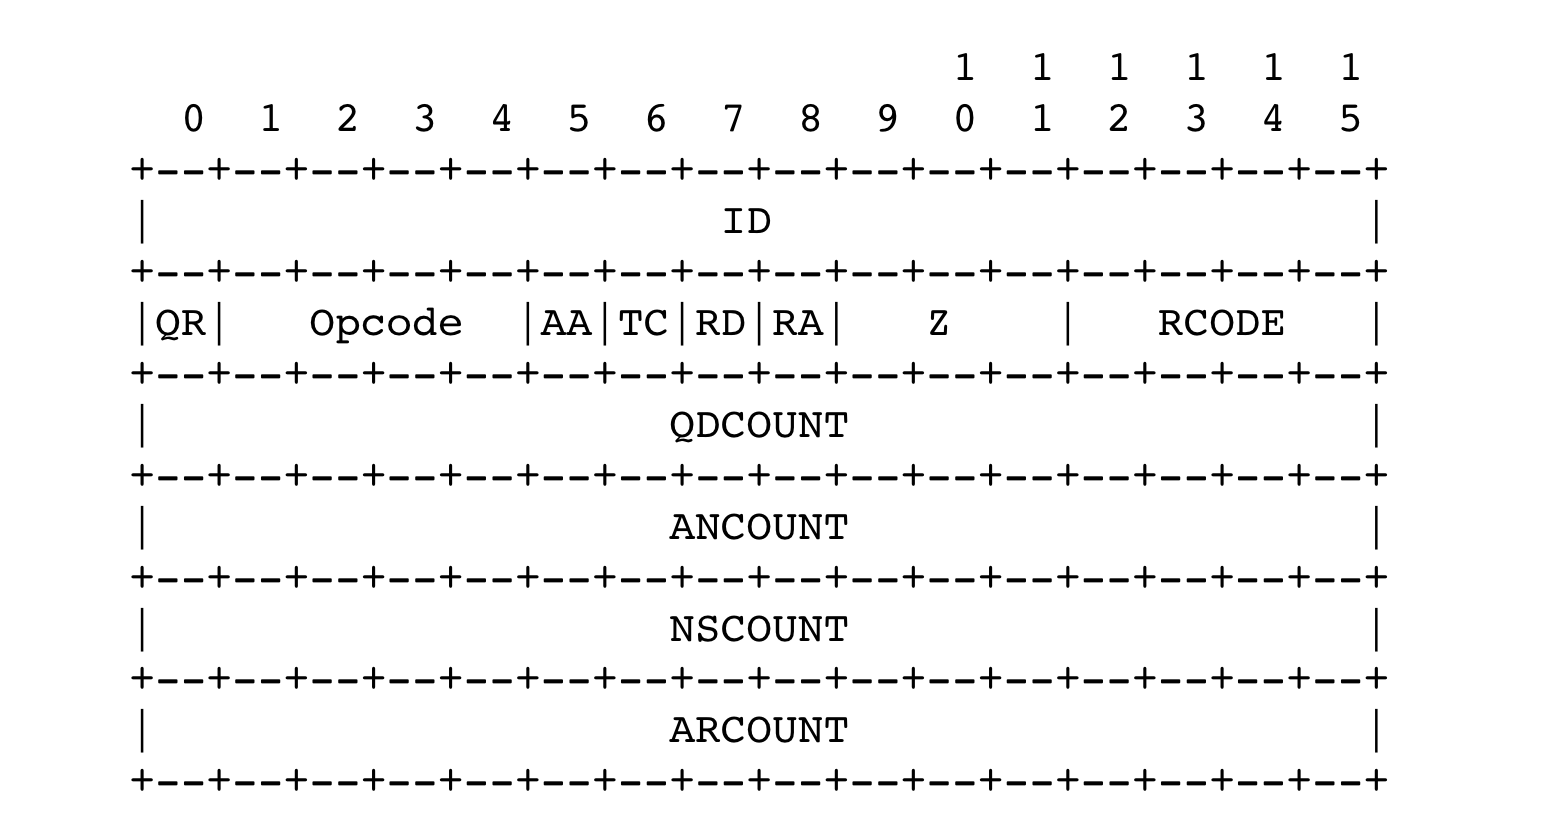
\includegraphics[width=10cm]{dns-header}
\centering
\caption{4.1.1. Header section format | RFC 1035}
\end{figure}

\textbf{DNS Header} has a fixed length, therefore its data structure representation can be easily casted upon the raw data.
Header includes significant meta data about the message, such as the number of questions and answers it carries 
or whether the message is a query or a response or even flags signaling corrupted or invalid messages.
This can be used for more directed parsing and filtering out those messages that this project doesn't care about.

\vspace{1cm}
\begin{figure}[h]
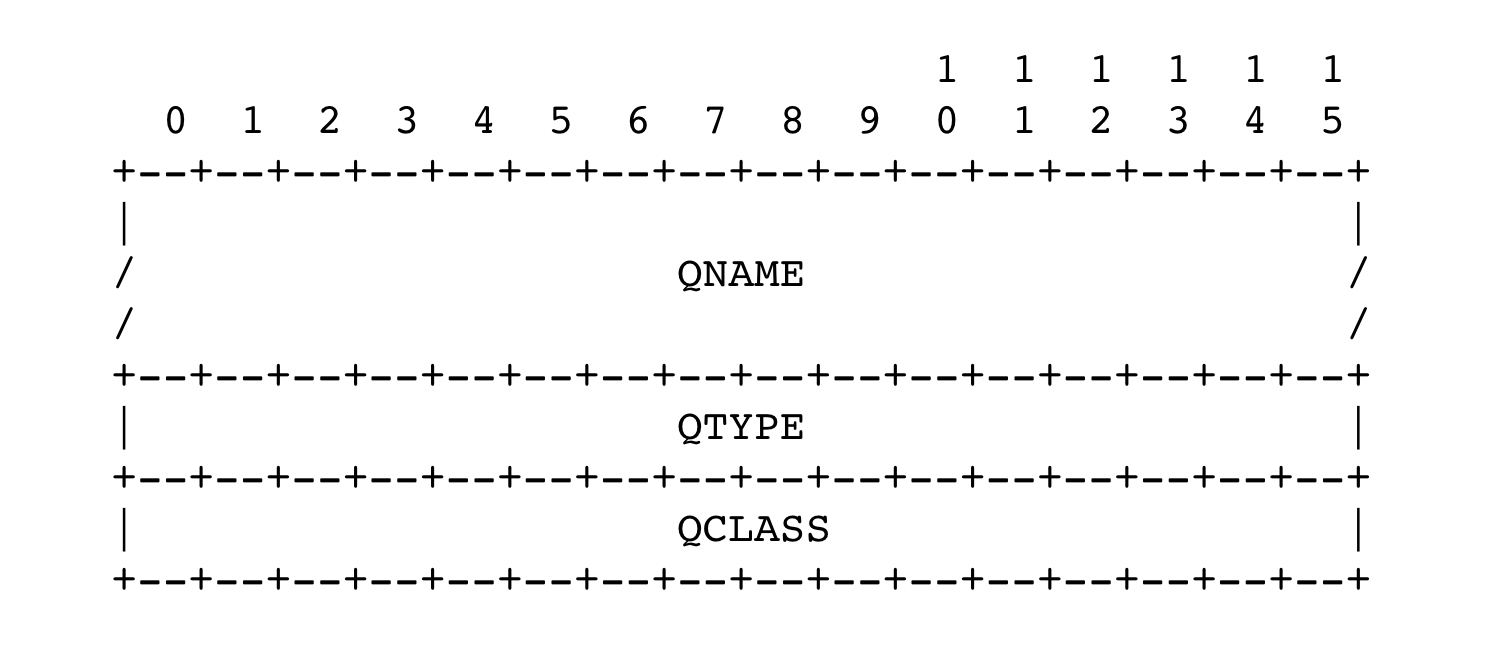
\includegraphics[width=10cm]{dns-question}
\centering
\caption{4.1.2. Question section format | RFC 1035}
\end{figure}

\textbf{Question section} of every DNS packet should contain an initial query record. 

Queries records contain three fields: \textit{QNAME}, \textit{QTYPE} and \textit{QCLASS}.

\vspace{1cm}
\begin{figure}[H]
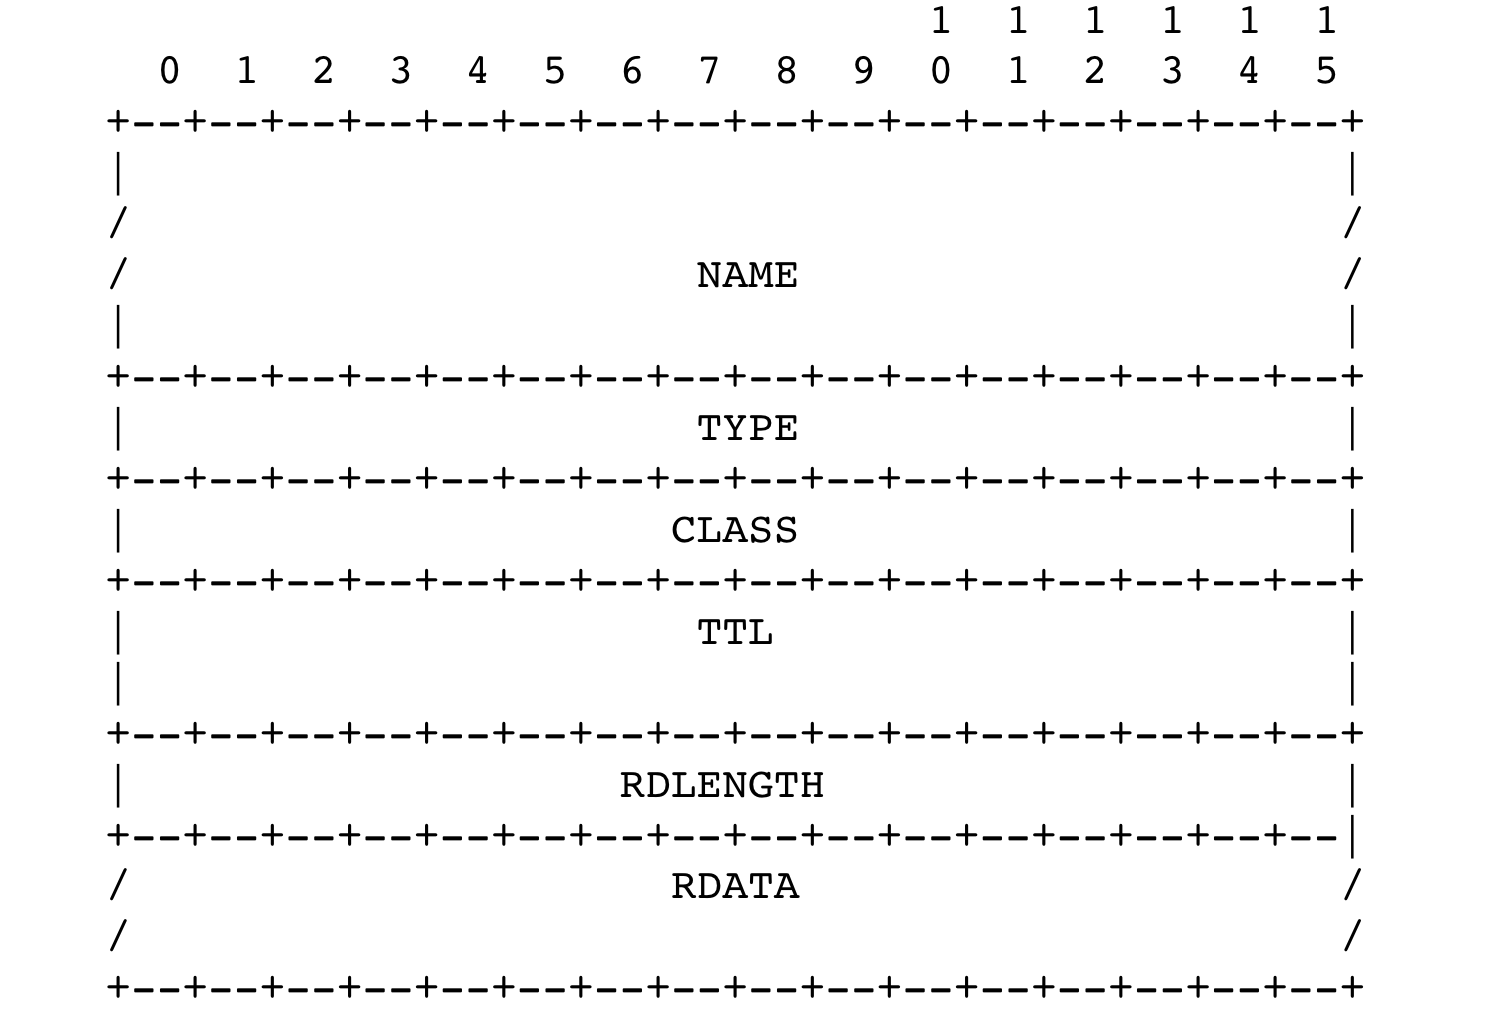
\includegraphics[width=8cm]{dns-rr}
\centering
\caption{4.1.3. Resource record format | RFC 1035}
\end{figure}

\textbf{Answer section} is the most meaningful section of a DNS message, as it contains the valuable response/responses for each query.
Answer sections shares the same format of resource records as the two other sections following it (Authority and Additional), however they are not used in this project.
Answers contain three fields: \textit{NAME}, \textit{TYPE}, \textit{CLASS}, \textit{TTL}, \textit{RDLENGTH} and \textit{RDATA}.

\textbf{RDATA} holds the actual response value during a DNS communication.
It can be represeted in various formats according to the DNS message type.

In this project, these DNS record types will be supported:
\begin{itemize}
\item \textbf{A} - Address record 
\item \textbf{AAAA} - IPv6 address record
\item \textbf{CNAME} - Canonical name record
\item \textbf{NS} - Name server record
\item \textbf{SOA} - Start of authority record
\item \textbf{PTR} - Pointer record
\item \textbf{MX} - Mail exchange record
\item \textbf{TXT} - Text record
\item \textbf{RRSIG} - DNSSEC signature
\item \textbf{NSEC} - Next Secure record
\item \textbf{DS} - Delegation signer
\item \textbf{DNSKEY} - DNS Key record
\end{itemize}

\vspace{0.5cm}

For all of these records, there is a specific parser implemented. 
The parser will output a string in a readable format and together 
with the message's question name and type, will be stored in a statistics collection.
If the same DNS resource record will be collected multiple times, 
it's count will increase rather than being inserted into the collection redundantly.

\pagebreak

\textbf{Exporting to a Syslog server}

The final task is to export collected statistics one by one to a foreign syslog server, if it was specified.
This simply means, that the application will create a new UDP socket, on which it will send simple messages 
in the official Syslog format specified in RFC 5424.

\subsection{Requirements}

Functional requirements from the assignment.
\begin{table}[H]
\centering
\caption{Requirements}
\label{my-label}
\resizebox{\textwidth}{!}{%
\begin{tabular}{@{}|l|l|@{}}
\toprule
\textbf{ID} & \textbf{DESCRIPTION} \\ \midrule
\textit{REQ\_01} & Aplication will process DNS protocol packets. \\ \midrule
\textit{REQ\_01\_01a} & Application will parse relevant link layer protocols (Ethernet, Linux SLL) \\ \midrule
\textit{REQ\_01\_01b} & Application will skip other link layer protocol types. \\ \midrule
\textit{REQ\_01\_02a} & Application will parse relevant network layer protocols (IPv4, IPv6) \\ \midrule
\textit{REQ\_01\_02b} & Application will skip other network layer protocol types. \\ \midrule
\textit{REQ\_01\_03a} & Application will parse relevant transport layer protocols (UDP, TCP) \\ \midrule
\textit{REQ\_01\_03b} & Application will skip other transport layer protocol types. \\ \midrule
\textit{REQ\_01\_04a} & Application will parse just DNS protocol on the application layer. \\ \midrule
\textit{REQ\_01\_04b} & Application will skip other application protocol types. \\ \midrule
\textit{REQ\_01\_05a} & Application will parse A, AAAA, CNAME, MX, NS, SOA, TXT, SPF, DNSKEY, NSEC, RRSIG and DS record types \\ \midrule
\textit{REQ\_01\_05b} & Application will skip other record types. \\ \midrule
\textit{REQ\_02} & Application will collect statistics about selected DNS messages. \\ \midrule
\textit{REQ\_02\_01} & Statistics will take this form: domain-name rr-type rr-answer count \\ \midrule
\textit{REQ\_03} & Application will export statistics to a specified syslog server. \\ \midrule
\textit{REQ\_04} & Application will be run as a executable in CentOS environment from the command line \\ \midrule
\textit{REQ\_05} & Application must accept arguments {[}-r file.pcap{]} {[}-i interface{]} {[}-s syslog-server{]} {[}-t seconds{]} \\ \midrule
\textit{REQ\_05\_01} & Application accepts -h argument for help \\ \midrule
\textit{REQ\_06} & Application will act accordingly to specified arguments \\ \midrule
\textit{REQ\_06\_01} & If interface argument is set, application will listen on a network interface. \\ \midrule
\textit{REQ\_06\_01\_01} & If syslog-server argument is also set, application will export statistics in regular intervals. \\ \midrule
\textit{REQ\_06\_01\_01a} & If seconds argument is also set, interval of statistics exporting is defined by this argument. \\ \midrule
\textit{REQ\_06\_01\_01b} & If seconds argument is not set, interval of statistics exporting is implicitly 60 seconds. \\ \midrule
\textit{REQ\_06\_01\_02} & If syslog-server argument is not set, application will ???? TODO \\ \midrule
\textit{REQ\_06\_02} & If file argument is set, application will read from a static .pcap file. \\ \midrule
\textit{REQ\_06\_02\_01} & Application should accept only .pcap files, or return error when pcap analysis doesn't accept the file. \\ \midrule
\textit{REQ\_06\_02\_02} & If syslog-server argument is also set, application will export statistics at the end of analysis. \\ \midrule
\textit{REQ\_06\_02\_03} & If syslog-server argument is not set, application will print out statistics to the standard output at the end of analysis. \\ \midrule
\textit{REQ\_06\_03} & Combination of interface and file arguments is forbidden. \\ \midrule
\textit{REQ\_06\_03} & Combination of file and seconds arguments is forbidden. \\ \midrule
\textit{REQ\_07} & Application will handle SIGUSR1 signal and print statistics to the standard output. \\ \midrule
\textit{REQ\_08} & Application will handle SIGINT signal and exit. \\ \midrule
\textit{REQ\_09} & Application will create syslog messages from collected statistics. \\ \midrule
\textit{REQ\_09\_01} & Syslog messages will be constructed with syntax according to RFC 5424 \\ \midrule
\textit{REQ\_09\_02} & Required fields are: timestamp, hostname, priority, version, executable name and the actual message data \\ \midrule
\textit{REQ\_09\_03} & Facility must be set to local0. \\ \midrule
\textit{REQ\_09\_04} & Severity must be set to Informational. \\ \midrule
\textit{REQ\_09\_05} & Application will send each statistic in a separate syslog message. \\ \midrule
\end{tabular}%
}
\end{table}

\pagebreak

\subsection{Solution}

Programming language used for the implementation: \textbf{C++} in a \textit{C++11 standard}.

Final solution is in my opinion complete, satisfying all the specified requirements in the previous section.
